\section[Fundamental Concepts]{\hyperlink{toc}{Fundamental Concepts}}
\subsection{The Beginnings of Quantum Mechanics}
Before we dive headfirst into the formalism of quantum mechanics, let us first review the first steps of the field as taken in the early 1900s. 

Our first founder is Max Planck; the problem at hand was the problem of the blackbody radiation spectrum. The two pre-existing laws (derived from thermodynamics arguments alone) predicting the BBR intensity as a function of wavelength/frequency were flawed. The first was Wien's law (1896):
\begin{equation}
    I_{\text{Wien}}(\lambda, T) \sim \frac{1}{\lambda^5}\exp(-\frac{1}{\lambda T}) % I(\lambda, T) = \frac{2hc^2}{\lambda^5}e^{-\frac{hc}{\lambda k_B T}}
\end{equation}
which agreed with low wavelength/high frequency data well but failed to accurately describe high wavelength/low frequency emission. The second was Rayleigh-Jeans' law (1900):
\begin{equation}
    I_{\text{RJ}}(\lambda, T) \sim \frac{T}{\lambda^4} % I(\lambda, T) = \frac{2ck_B T}{\lambda^4}
\end{equation}
which agreed with high wavelength/low frequency data well but failed to accurately describe low wavelength/high frequency emission\footnote{It should be noted however that a full-derivation of the Rayleigh-Jeans law did not occur until 1905, at which point Planck had already established the more correct explanation.}. In fact, the intensity as predicted by Rayleigh-Jeans' diverges at low $\lambda$, leading to the (obviously) erroneous conclusion that the total energy emitted by a black body is infinite; the so-called ``ultraviolet catastrophe''.

In order to solve this problem, in 1900 Planck proposed a quantum hypothesis; that light carries energy in individual packets, or quanta. In particular, for light of frequency $f$, each quanta carries energy:
\begin{equation}
    E = hf.
\end{equation}
Combining this quantum hypothesis with the Boltzmann supression of high-energy states (from thermodynamics), Planck's law was then derived to be:
\begin{equation}
    I_{\text{Planck}}(\lambda, T) = \frac{2hc^2}{\lambda^5}\frac{1}{\exp(\frac{hc}{\lambda k_B T}) - 1}
\end{equation}
which agrees with the BBR spectrum data across all frequencies\footnote{Further, we can observe that Planck's law agrees with Wien's law in the high-frequency limit, and with Rayleigh-Jeans' law in the low-frequency limit.}. It should also be noted that the integral over all $f$ of the above radiance law yields is finite, resolving the ultraviolet catastrophe. 

\begin{figure}[htbp]
    \centering
    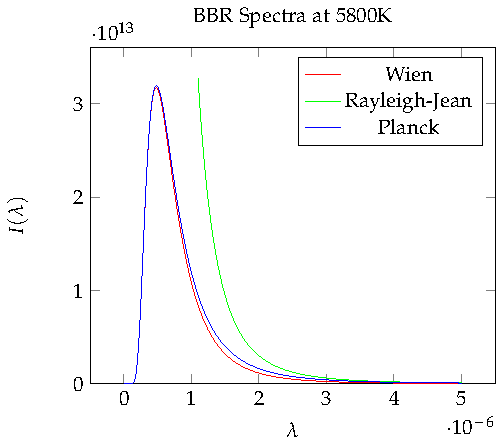
\includegraphics[]{Images/fig-BBRspectra.pdf}
    \caption{Plots of the black body emission spectra at $T = 5800\mathrm{K}$ (the approximate temperature of the surface of the sun) as predicted by Wien's Law, Rayleigh-Jean's Law, and Planck's Law. Planck's Law was found to agree with experimental observations for all wavelengths. Wien's Law agrees with observations well in the short wavelength limit but fails for long wavelengths. Rayleigh-Jean's Law agrees with observations in the long wavelength limit but fails at short wavelengths, and in fact the predicted emitted energy diverges.}
    \label{fig-BBRspectra}
\end{figure}


\noindent
In the above discussion, we have introduced Planck's constant. It has numerical value\footnote{which is the set/absolute (rather than measured) value of the Planck constant as per the 2018 redefinition of SI units.}:
\begin{equation}
    h = 6.626070040 \times 10^{-34}\si{J.s}
\end{equation}
$h$ is quantified as ``small''. What exactly does small mean in this context? For comparison, $1\si{eV}$ is the kinetic energy of an electron acquired in a voltage drop of a Volt, $0.035\si{eV}$ is the average kinetic energy of an atom at room temperature (from $E_k = \frac{3}{2}k_B T$) and $2.4\si{eV}$ is the energy of a single photon from the middle of the visible spectrum ($600 \si{THz}$). The energy of a single photon, which depends on $h$, is in other words ``typical'' of microscopic phenomena.

Planck's quantum hypothesis would be confirmed in Einstein's (Nobel-prize winning) 1905 explanation of the photoelectric effect (which you likely covered in detail in a previous course in modern physics); namely that quanta of light transfer energy $E = hf$ to electrons in the metal, kicking them out\footnote{Provided of course that $hf > \Phi$ where $\Phi$ is the ``work function'' of the metal.}.

Our second founder of interest is DeBroglie. In 1924, he postulated that matter could behave like a wave, positing the DeBroglie wavelength relation:
\begin{equation}
    p = \frac{h}{\lambda}.
\end{equation}
The so-called ``wave-particle'' duality would be confirmed in 1927 by the Davisson-Germer experiment, which saw peaks of electron intensity at distinct angles, showing that electrons scatter in the same nature as photons.

Our third founder of interest is Schr\"{o}dinger, who postulated the Schr\"{o}dinger equation (expressed below in the position basis) in 1926:
\begin{equation}
    i\hbar \dpd{}{t}\psi(\v{r}, t) = \left[\frac{-\hbar^2}{2m}\nabla^2 + V(\v{r}, t)\right] \psi(\v{r}, t).
\end{equation}
It should be noted that this is one of the two core formulas of non-relativistic quantum mechanics, and is the quantum-mechanical equivalent of Newton's laws. It however does not cover the effects of special relativity (for which we defer the reader to a future course on quantum field theory) or quantum measurement (which we shall address now). 

An illuminating demonstration of quantum measurement takes the form of the Stern-Gerlach experiment (first carried out in 1921/1922; see \href{https://physicstoday.scitation.org/doi/10.1063/1.1650229}{this article} for more historical background). In this experiment, silver atoms are heated and escape from an oven with uniform velocity. The beam of atoms then pass through an inhomogenous magnetic field (generated by an asymmetric pair of magnetic pole pieces) where they are deflected, before hitting a screen where their position is recorded. 

\begin{figure}[htbp]
    \centering
    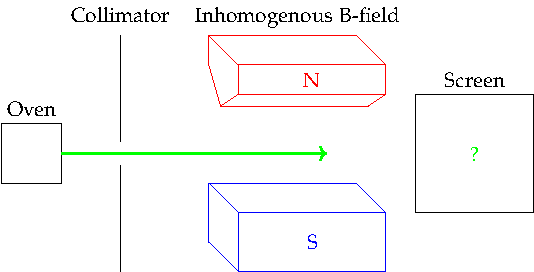
\includegraphics[]{Images/fig-SGexpsketch.pdf}
    \caption{Illustration of the Stern-Gerlach experiment. Silver (Ag) atoms are heated in an oven and escape, and pass through a collimator to form a narrow beam. They then pass through an inhomogenous magnetic field which deflects the atoms. The position of the atoms is then recorded when they hit the screen.}
    \label{fig-SGexpsketch}
\end{figure}

Why are silver atoms used for this experiment? Moreover, what exactly is being measured? For this, we consider a simplified model of the atom (which will suffice for the purposes of explaining this experiment). Silver atoms consist of 47 electrons in the shell, and 47 protons and 61 neutrons in the nucleus. A first guess of the mechanism of the atoms being deflected by the magnetic field may be a Lorentz force effect; however this is not the case as the atoms are electrically neutral. Instead, the silver atom has a single unpaired electron which has an intrinsic angular momentum, known as spin. In particular, the electron is spin-1/2\footnote{We will return to a more detailed discussion of angular momentum and spin at a later portion of the course}. This provides the silver atom with a net magnetic moment $\gv{\mu}$ proportional to the electron spin\footnote{The astute reader may question why the spin of the unpaired proton in the nucleus has no contribution to the net magnetic moment. This is due to the fact that the proportionality factor between the spin and magnetic moment has a factor of inverse mass. Since the proton is 1836 times heavier than the electron, the proton's magnetic moment contribution is negligeble compared to the electron's.} $\v{S}$:

\begin{equation}
    \gv{\mu} \propto \v{S}.
\end{equation}
We then recall from electromagnetism that a magnetic dipole $\gv{\mu}$ in a magnetic field $\v{B}$ has interaction energy:
\begin{equation}
    E = -\gv{\mu} \cdot \v{B}.
\end{equation}
We can then find the force that the dipole feels by taking the (negative) gradient of the energy:
\begin{equation}
    \v{F} = -\gv{\nabla}(-\gv{\mu} \cdot \v{B}) = \mat{\dpd{}{x}(\gv{\mu} \cdot \v{B}) \\ \dpd{}{y}(\gv{\mu} \cdot \v{B}) \\ \dpd{}{z}(\gv{\mu} \cdot \v{B})}.
\end{equation}
Ignoring the magnetic fields that are not in the $z$-direction, we find the force on the silver atoms in the $z$-direction to be:
\begin{equation}
    F_z = \mu_z \dpd{B_z}{z}.
\end{equation}
So in the inhomogenous field produced by the asymmetric magnets, the silver atoms should feel an up/downwards force depending on the direction of $\v{S}$ (which determines $\mu_z$). 

\begin{figure}[htbp]
    \centering
    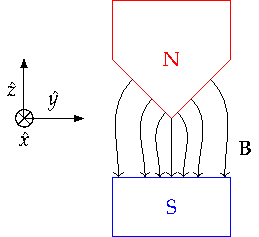
\includegraphics[]{Images/fig-SGexpmagnet.pdf}
    \caption{The inhomogenous magnetic field used in the Stern-Gerlach experiment, which deflects the silver atoms due to their magnetic dipole moment proportional to electron spin.}
    \label{fig-SGexpmagnet}
\end{figure}

Classically, the magnetic moment $\v{\mu}$ can point in any direction, and therefore $\mu_z$ ranges continuously from $+\abs{\gv{\mu}}$ to $-\abs{\gv{\mu}}$. Hence, the signature we would expect on the Stern-Gerlach experiment screen (wherein the vertical position of the atoms on the screen corresponds to a measurement of the $z$-component of the magnetic moment) would be a continuous band, as seen in the left of Fig. 1.4 below. However, this is \emph{not} what is observed; instead the experimental result was two discrete dots with nothing in between, as seen in the right of the figure. 

\begin{figure}[htbp]
    \centering
    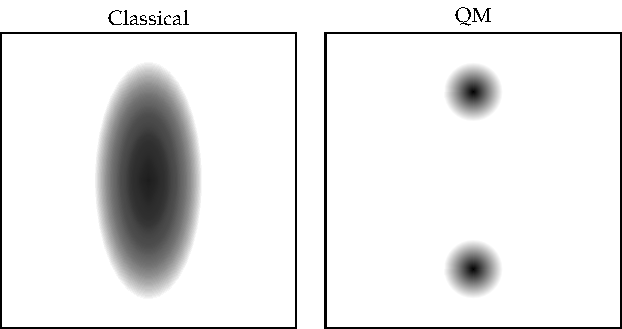
\includegraphics[]{Images/fig-SGexppredictions.pdf}
    \caption{Classical prediction (left) and quantum mechanical prediction (right) for the Stern-Gerlach experiment. The screen on the right was observed in experiment.}
    \label{fig-SGexppredictions}
\end{figure}

How do we interpret this result? We can associate the top dot with spins fully polarized upwards ($\uparrow$) and the bottom dot with spins fully polarized downwards ($\downarrow$). But why is there no signature for sideways pointing spins? We first will answer how a general spin (1/2) state can be represented. If $\ket{\uparrow}$ represents the spin-up state and $\ket{\downarrow}$ represents the spin-down state, then a general spin (and hence sideways spins) can be represented as complex superpositions of these two states, i.e.
\begin{equation}
    \ket{\psi} = \alpha\ket{\uparrow} + \beta\ket{\downarrow}
\end{equation}
where $\alpha, \beta \in  \CC$. What happens in a measurement is then that one element of this general superposition is picked with some probability; indeed, quantum measurement is a probabilistic process. Specifically, we find according to the Born rule that the probability that we measure the spin to be up is $p(\uparrow) = \abs{\uparrow}^2$ and the probability that we measure the spin to be down is $p(\downarrow) = \abs{\downarrow}^2$. Since we require that we measure either spin-up or spin-down, we obtain the normalization condition:
\begin{equation}
    p(\uparrow) + p(\downarrow) = \abs{\alpha}^2 + \abs{\beta}^2 = 1.
\end{equation}
The spin state after the measurement is then $\ket{\uparrow}$ or $\ket{\downarrow}$ respectively, according to the Dirac projection postulate. We will return to these two postulates of quantum mechanics and discuss them in full generality shortly. 

However, we will however make a second comment about measurement before concluding this section. Namely, we consider the case where we perform a repeated measurement of the $z$-component of the spin. As discussed above, the initial general spin state is given by $\ket{\psi} = \alpha\ket{\uparrow} + \beta\ket{\downarrow}$. We then measure the $z$-component of spin and the post-measurement spin state is $\ket{\uparrow}$ or $\ket{\downarrow}$ with probability $\abs{\alpha}^2$ and $\abs{\beta}^2$ respectively. What happens if we measure the $z$-component of spin again? We might think that again, we have probability $\abs{\alpha}^2$ of measuring spin-up and probability $\abs{\beta}^2$ of measuring spin-down. But this is \emph{not} the case. If we measured spin-up in the first measurement, we will measure spin-up in the second measurement with probability one. Similarly, if we measured spin-down in the first measurement, we will measure spin-down in the second measurement with probability one. Evidently, the first measurement has done something to the spin such that the measurement probabilities for the second measurement have been affected (they are not the same as the first). This tells us that quantum measurement is a active process that influences the state of the system we measure. Specifically, it is an irreversible process; there is no notion of ``undo''-ing the measurement to recover the initial (pre-measurement) state.


\subsection{Kets, Bras, and Hilbert Space}
Our goal of the initial stages of this course will be to understand the following table:

\begin{table}[htbp]
    \centering\begin{tabular}{|c|c|}
        \hline Quantum states & $\ket{\psi} \in \H$ 
        \\ \hline Evolution & $i\hbar\pd{}{t}\ket{\psi} = H\ket{\psi}$
        \\ \hline Measurement & $\ket{\psi} \mapsto \frac{\Pi_j \ket{\psi}}{\sqrt{\bra{\psi}\Pi_j\ket{\psi}}} \quad p(j) = \bra{\psi}\Pi_j\ket{\psi}$
        \\ \hline
    \end{tabular}
    \caption{Axioms of quantum mechanics, concerning states, evolution, and measurement.}
    \label{table-QMaxioms}
\end{table}

We will discuss the axioms for quantum states and quantum measurement in this chapter, and the axiom for quantum evolution (which readers may recognize as the Schr\"{o}dinger equation in basis independent form) in the next. It is worth noting that these are the \emph{fundamental postulates} of quantum mechanics; like Newton's laws of motion in classical mechanics, they cannot be derived. We are only able to interpret them, check if they are consistent, and work out the implications.

Let's start the axiom for quantum states; after all it will helpful to know what the objects of our interest are, before we start to work with them! 

\begin{axiombox}{: Quantum states}\label{axiom-states}
    Quantum states $\ket{\psi}$ are vectors (also called ``kets'') in a complex Hilbert space $\H$.
\end{axiombox}

The above axiom is only meaningful if we know what a Hilbert space is; its definition is below:

\begin{defbox}{: (Complex) Hilbert spaces}\label{def-Hilbertspaces}
    $\H$ is a (complex) Hilbert space if:
    \begin{enumerate}[(i)]
        \item $\H$ is a vector space over $\CC$
        \item $\H$ has an inner product
        \item $\H$ is complete (with respect to the metric induced by the norm induced by the inner product)\footnotemark - For the purposes of this course, this last point can be ignored.
    \end{enumerate}
\end{defbox}
\footnotetext{This is a technical qualification for the mathematicians in the crowd. An intuitive explanation for the curious; the inner product on a Hilbert spaces creates a notion of distance on the space. There are sequences (of vectors) that get closer together over time; completeness tells us that any such sequences (known as Cauchy sequences) must converge to a limit.}

Note that the vector space axioms for closure imply that $\forall \ket{\psi}, \ket{\phi} \in \H$ (where $\forall$ means ``for all'') and $\forall c \in \CC$, then $\ket{\psi} + \ket{\phi} \in \H$ and $c\ket{\psi} \in \H$. This tells us that the superposition of quantum states is well defined!

An example which we will return to time and time again (and have already encountered once) is the Hilbert space for a spin-1/2 system. In this case, $\H = \CC^2$. A question that may be brooding in the reader's mind may be ``why do we have to use complex numbers?''; one may indeed wonder if real Hilbert spaces may suffice to do quantum mechanics. The response is negative; we indeed need complex numbers! As an illustrative example, consider again the general spin-1/2 state $\ket{\psi} = \alpha\ket{\uparrow} + \beta\ket{\downarrow}$. Suppose we want a state that has equal probability to be measured spin-up or spin-down under a measurement of the $z$-component of spin. Since $p(\uparrow) = \abs{\alpha}^2$ and $p(\downarrow) = \abs{\beta}^2$, in order to have equal probability we must have $\abs{\alpha} = 1/\sqrt{2}$ and $\abs{\beta} = 1/\sqrt{2}$. A spin pointing in the $+x$ or $-x$ directions indeed has equal weight of up and down. Up to an overall (irrelevant) minus sign, without using complex numbers there are two ways to superimpose $\ket{\uparrow}$ and $\ket{\downarrow}$, from which we can define states corresponding to spins fully polarized in $\pm x$:

\begin{equation}\label{eq-xpm}
    \ket{x, \pm} = \frac{\ket{\uparrow} \pm \ket{\downarrow}}{\sqrt{2}}.
\end{equation}
However, the $\pm \hat{x}$ and $\pm \hat{y}$ vectors lie in the same $z = 0$ plane, and by symmetry we should require that the $\ket{y, \pm}$ would also have equal weights of $\ket{\uparrow}$ and $\ket{\downarrow}$. But if we limit ourselves to real numbers only, we have already exhausted all possible equal-weight combinations of $\ket{\uparrow}$ and $\ket{\downarrow}$ in Eq. \eqref{eq-xpm}. We therefore require complex  numbers to represent all possible states (and indeed, we find that $\ket{y, \pm} = \frac{\ket{\uparrow} \pm i \ket{\downarrow}}{2}$).

Having motivated the ``complex'' in the complex vector space part of the definition of Hilbert spaces, let us now motivate the inner product. We want some way to compare quantum states to one another. Our geometric intuition tells us that the states $\ket{\uparrow}$ and $\ket{\nearrow}$ are ``close'' to each other, while $\ket{\uparrow}$ and $\ket{\downarrow}$ are very ``different''. In order to make this intuition rigorous, we define the inner product, and as a prerequisite we define the dual correspondence.

\begin{defbox}{: Dual correspondence}\label{def-dualcorrespondence}
    To each vector space $\H$, there exists a dual vector space $\H^*$. There is a one-to-one correspondence\footnotemark between the kets $\ket{\psi} \in \H$ and the bras\footnotemark $\bra{\psi} \in \H^*$. We call this the \emph{dual correspondence}, and write it as follows:
    \begin{equation}
        \ket{\psi} \DC \bra{\psi}.
    \end{equation}
    It has the following properties:
    \begin{enumerate}[(i)]
        \item $\ket{\psi} + \ket{\phi} \DC \bra{\psi} + \bra{\phi}$
        \item $c\ket{\psi} \DC c^*\bra{\psi}$
    \end{enumerate}
    where the $*$ denotes complex conjugation.
\end{defbox}
\footnotetext{Formally, this follows from the Riesz Representation Theorem. But for the purposes of this course, we take this one-to-one correspondence as a postulate. Curious readers can find discussions/proofs of the theorem in any text on functional analysis, or mathematical quantum theory.}
\footnotetext{Given such names because $\braket{}{}$ is a bracket - bra-ket. Physicists remain unmatched in their sense of humour.}

Having established the dual correspondence, we may now define the inner product:

\begin{defbox}{: Inner product}\label{def-innerproduct}
    We define the inner product between $\ket{\psi} \in \H$ and $\ket{\phi} \in \H$ as:
    \begin{equation}
        \braket{\phi}{\psi} \in \CC
    \end{equation}
    with the properties:
    \begin{enumerate}[(i)]
        \item $\braket{\phi}{\psi} = \braket{\psi}{\phi}^*$
        \item $\braket{\psi}{\psi} \geq 0, \forall \ket{\psi} \in \H$
        \item $\braket{\psi}{\psi} = 0 \implies \ket{\psi} = \v{0}$.
    \end{enumerate}
\end{defbox}
Note that $\v{0}$ in the above definition is the null ket (also known as the zero vector, which must be an element of the Hilbert space), where $\v{0} = 0\ket{\psi}, \forall \ket{\psi}$. It is an unphysical state. We normally work with normalized states, i.e. states $\ket{\psi}$ that satisfy $\braket{\psi}{\psi} = 1$. The null ket has inner product zero and cannot be normalized.

As a first use of the inner product, let us return to our initial motivation for obtaining the ``likeness'' of states. For normalized states, it follows (and we will later prove) that:
\begin{equation}
    0 \leq \abs{\braket{\phi}{\psi}} \leq 1.
\end{equation}
We therefore can use the inner product as a method to evaluate the likeness of states. $\braket{\phi}{\psi} = 0$ means that $\ket{\psi}$ and $\ket{\phi}$ are maximally different, and $\abs{\braket{\phi}{\psi}} = 1$ corresponds to $\ket{\psi}$ and $\ket{\phi}$ being the same.

Next, we move onto a discussion of bases of Hilbert spaces. Since Hilbert spaces are vector spaces, they admit a basis. Let us recall what a basis is.

\begin{defbox}{: Basis}\label{def-basis}
    A \emph{basis} $\mathcal{B}$ of $\H$ is a set of states $\mathcal{B} = \set{\ket{b_j}}_j$ such that every state $\ket{\psi} \in \H$ can be written in the form:
    \begin{equation}\label{eq-expandpsibasis}
        \ket{\psi} = \sum_j \psi_j \ket{b_j}
    \end{equation}
    with $\psi_j \in \CC \forall j$, and the expansion on the RHS is unique.

    $\abs{\mathcal{B}}$ is the dimension of $\mathcal{H}$\footnotemark. 
\end{defbox}
\footnotetext{In the case where the Hilbert space is infinite-dimensional, there are additional complications (and in fact, two different kinds of bases!) In general the work we do in this course works perfectly well in the finite-dimensional case, and in the infinite dimensional case we will have to wave our hands a bit in order to avoid getting into the weeds of functional analysis; this is a physics course after all.}

Of particular interest to us will be orthonormal bases, or ONBs.

\begin{defbox}{: Orthonormal bases}\label{def-ONB}
    A basis $\mathcal{B} = \set{\ket{b_j}}_j$ is \emph{orthonormal} if
    \begin{equation}
        \braket{b_i}{b_j} = \delta_{ij}.
    \end{equation}
    where $\delta_{ij}$ is the Kronecker delta, defined as:
    \begin{equation}
        \delta_{ij} = \begin{cases}
            1 & i = j
            \\ 0 & i \neq j
        \end{cases}.
    \end{equation}

    One can obtain the expansion coefficients $\psi_j$ with respect to ONBs. Writing $\ket{\psi} = \sum_j \psi_j \ket{b_j}$ as in Eq. \eqref{eq-expandpsibasis} and taking the inner product of $\ket{\psi}$ with a vector $\ket{b_i}$ from the ONB, we have:
    \begin{equation}
        \braket{b_i}{\psi} = \sum_j \psi_j \braket{b_i}{b_j} = \sum_j \psi_j \delta_{ij} = \psi_i.
    \end{equation}
\end{defbox}

We will now prove a useful trick involving ONBs.

\begin{thmbox}{: Resolution of the identity}\label{thm-residentity}
    For all ONBs $\set{\ket{b_j}}_j$, the following relation holds:
    \begin{equation}
        \sum_j \dyad{b_j}{b_j} = \II
    \end{equation}
    where $\II$ is the identity operator on the Hilbert space.
\end{thmbox}

\begin{proof}
    Recall that $\ket{\psi} = \sum_j \psi_j \ket{b_j}$ for any $\ket{\psi} \in \H$ and for any basis $\set{\ket{b_j}}_j$ of $\H$. Further, recall that $\psi_j = \braket{b_j}{\psi}$ if the basis is orthonormal. Hence we have that:
    \begin{equation}
        \ket{\psi} = \sum_j \braket{b_j}{\psi}\ket{b_j} = \sum_j \ket{b_j}\left(\braket{b_j}{\psi}\right) = \sum_j \left(\dyad{b_j}{b_j}\right)\ket{\psi} = \left(\sum_j \dyad{b_j}{b_j}\right)\ket{\psi}.
    \end{equation}
    Since the above relation holds for all $\ket{\psi}$, it follows then that $\sum_j\dyad{b_j}{b_j}$ is the identity as claimed.
\end{proof}

At this point in the course, the reader may be wondering what happened to quantum \emph{wavefunctions}\footnote{Though this nomenclature of ``wavefunction'' is arguably a misnomer; the Schr\"{o}dinger equation does not contain second order derivatives in time, as a wave equation would.}; the central objects of interest have instead been quantum states, without a wavefunction in sight. We now elucidate the connection between the two.

\begin{defbox}{: Wavefunctions}
    Consider (as before) expanding $\ket{\psi}$ in a ONB $\set{\ket{b_j}}_j$. We then have:
    \begin{equation}
        \ket{\psi} = \sum_j \ket{b_j}\braket{b_j}{\psi}.
    \end{equation}
    Therein, $\psi_j = \psi(j) = \braket{b_j}{\psi}$ is the \emph{wavefunction}; a wavefunction is just a quantum state expanded in a given ONB. 
\end{defbox}

A particularly important (and familiar) example is using the position basis. Consider the resolution of the identity involving position:
\begin{equation}
    \int \mathrm d x \dyad{x}{x} = \II.
\end{equation}
For any $\ket{\psi}$, we then have:
\begin{equation}
    \ket{\psi} = \int \mathrm d x \ket{x}\braket{x}{\psi}.
\end{equation}
Where $\braket{x}{\psi} = \psi(x)$ is the position wavefunction, which played a central role in your first course in quantum mechanics. However, the reader should now recognize that $\ket{\psi}$ is a more fundamental object than this wavefunction, as it not only contains the information for $\psi(x)$ but also for $\tilde{\psi}(p)$ (the momentum wavefunction) or any other wavefunction; any wavefunction is just the expansion coefficients of the state in a given basis.

We have now established quite a bit of machinery to discuss quantum states, but have not done anything with the states; let's change that by discussing measurements! In a quantum measurement, the alternatives $\set{\ket{m_j}, j \in \text{ Outcomes }}$ for the states after measurement will:
\begin{itemize}
    \item Form a basis
    \item And are pairwise orthogonal, i.e. $\braket{m_i}{m_j} = 0, \forall i \neq j$. 
\end{itemize}
With the necessary mathematical formalism under our belt, we can now state a first version of the Dirac postulate and Born rule axioms.

\begin{axiombox}{: Quantum measurement (version 1)}\label{axiom-measurementver1}
    \textbf{Dirac postulate:} Under quantum measurement, the measured quantum state $\ket{\psi}$ is probabilistically changed into one of a number of alternatives $\set{\ket{m_j}}_j$, with:
    \begin{equation}
        \braket{m_i}{m_j} = \delta_{ij}.
    \end{equation}
    Note that $\set{\ket{m_j}}_j$ forms an ONB.
    
    \textbf{Born rule:} Given a quantum state $\ket{\psi}$, the probability for obtaining outcome $j$, corresponding to post-measurement state $\ket{m_j}$, is:
    \begin{equation}
        p_j = \abs{\braket{m_j}{\psi}}^2.
    \end{equation}
\end{axiombox}

There are now two questions that may arise. The first is that the statement of the Dirac projection postulate and the Born rule do not match that found in Table \ref{table-QMaxioms}. The second question concerns the post-measurement states $\set{\ket{m_j}}_j$; namely, how are they are determined? We will address the latter question first, and build up the formalism to state the measurement axioms in full generality. To this end, we move to a discussion of linear operators, which describe quantum mechanical observables and evolution. 

\subsection{Operators and Observables}

\begin{defbox}{: Linear Operators}\label{def-linops}
    $A$ is an \emph{operator} that acts on a Hilbert space $\H$ if $\forall \ket{\psi} \in \H$, $A\ket{\psi} \in \H$. $A$ is $\emph{linear}$ if:
    \begin{equation}
        A(\alpha\ket{\psi} + \beta\ket{\phi}) = \alpha(A\ket{\psi}) + \beta(A\ket{\phi})
    \end{equation}
    $\forall \ket{\psi}, \ket{\phi} \in \H$ and $\forall \alpha, \beta \in \CC$.
\end{defbox}

A point of notation; we will use capital letters to denote operators in this course. Some sources also use hats to denote this (e.g. $\hat{A}$). Note that linear operators can be added and multiplied (more accurately, composed) to yield other linear operators. They are associative and distributive under these operations, i.e. for all linear operators $A, B, C$ we have:
\begin{equation}
    (A + B) + C = A + (B + C)
\end{equation}
\begin{equation}
    (AB)C = A(BC)
\end{equation}
\begin{equation}
    A(B + C) = AB + AC.
\end{equation}
However, note that in general operators are \emph{not} commutative, that is:
\begin{equation}
    AB \neq BA.
\end{equation}

Quantum mechanical observables are a specific type of linear operators; namely, they are Hermitian. In order to make sense of this, we introduce two more definitions.

\begin{defbox}{: Hermitian adjoint}\label{def-adjoint}
    The \emph{Hermitian adjoint} $A^\dagger$ of a linear operator $A$ is defined via the dual correspondence:
    \begin{equation}
        A\ket{\psi} \DC \bra{\psi}A^\dagger.
    \end{equation}
\end{defbox}

\begin{defbox}{: Hermitian operators and observables}\label{def-observables}
    An operator $A$ is \emph{Hermitian} if:
    \begin{equation}
        A^\dagger = A.
    \end{equation}
    Quantum mechanical \emph{observables} (such as position, momentum, spin, and energy) are Hermitian operators.
\end{defbox}

In general, acting on a state with an operator changes the state, and the new state is not necessarily proportional to the original state, i.e:
\begin{equation}
    A\ket{\psi} \not\propto \ket{\psi}.
\end{equation}
However, for special states known as eigenstates of an operator, this is indeed the case.

\begin{defbox}{: Eigenstates and eigenvalues}\label{def-eigstates}
    An \emph{eigenstate} $\ket{a}$ of a linear operator $A$ is a state that satisfies:
    \begin{equation}
        A\ket{a} = a\ket{a}.
    \end{equation}
    Therein, $a \in \CC$ is the \emph{eigenvalue} corresponding to that eigenstate. The null vector $\v{0}$ is excluded from being an eigenvector.
\end{defbox}

Having defined these objects, we state (but do not prove) an important theorem concerning observables:

\begin{thmbox}{: Diagonalization/Spectral Theorem}
    A Hermitian operator $A$ (i.e. any observable) can be diagonalized; that is, it is able to be written as:
    \begin{equation}
        A = \sum_i a_i \dyad{a_i}{a_i}
    \end{equation}
    Where the eigenvectors $\set{\ket{a_i}}$ of $A$ forms an orthonormal basis\footnotemark (an \emph{eigenbasis}) and $a_i$ are the corresponding eigenvalues.
\end{thmbox}
\footnotetext{If the eigenvalues of $A$ are non-degenerate, then the set of eigenstates of $A$ are automatically mutually orthogonal, as we prove in the next theorem. If $A$ has degenerate eigenvalues, two eigenstates with the same eigenvalue are not necessarily guaranteed to be orthogonal, but we are still able to choose eigenstates (picking orthogonal vectors from the degenerate subspaces) to form an ONB out of the eigenstates; so we need not worry too much.}
With some more machinery developed, we can more carefully state the Dirac postulate and the Born rule.

\begin{axiombox}{: Quantum measurement (version 2)}
    \textbf{Dirac postulate:}
    \begin{enumerate}
        \item Each possible outcome of the measurement of an observable $A$ is an eigenvalue of $A$.
        \item If the eigenvalue $a$ is found in the measurement, then the post measurement state is an eigenvector $\ket{a}$ of $A$,
        \begin{equation}
            \ket{\psi} \mapsto \ket{a}
        \end{equation}
        satisfying
        \begin{equation}
            A\ket{a} = a\ket{a}.
        \end{equation}
    \end{enumerate}

    \textbf{Born rule:} Given an initial state of $\ket{\psi}$, the possibility for the measurement outcome $a_i$ occuring in a measurement of an observable $A$ (where $a_i$ is an eigenvalue of $A$) is:
    \begin{equation}
        p_i = \abs{\braket{a_i}{\psi}}^2.
    \end{equation}
\end{axiombox}

We reiterate that the eigenstate $\ket{a}$ is the possible post-measurement state, and the eigenvalue $a$ is the corresponding measurement outcome. As a concrete example, the spin-$z$ operator $S_z$ (for spin-1/2) systems has eigenstates $\ket{\uparrow}$ and $\ket{\downarrow}$, with corresponding eigenvalues of $+\hbar/2$ and $-\hbar/2$ (i.e. $S_z\ket{\uparrow} = +\hbar/2\ket{\uparrow}$, and likewise for $\ket{\downarrow}$). We may write $S_z$ in diagonal form as:
\begin{equation}
    S_z = \frac{\hbar}{2}(\dyad{\uparrow}{\uparrow} - \dyad{\downarrow}{\downarrow}).
\end{equation}
A measurement of the $z$ component of spin has two possible outcomes $\pm \hbar/2$, corresponding to post measurement states $\ket{\uparrow}/\ket{\downarrow}$. $\set{\ket{\uparrow}, \ket{\downarrow}}$ is an ONB, and we can expand a general state $\ket{\psi}$ in this basis as $\ket{\psi} = \alpha\ket{\uparrow} + \beta\ket{\downarrow}$. The Born rule then tells us that $p(\uparrow) = \abs{\braket{\uparrow}{\psi}}^2 = \abs{\alpha}^2$ and similarly that $p(\downarrow) = \abs{\beta}^2$. 

There are two points of consistency that the restatement of the Dirac postulate invites. First, an experiment should only have real-valued outcomes; an measurement shouldn't return a complex number. Second, it is not a priori immediate that the eigenstates/post-measurement states are mutually orthogonal, as the first statement of the postulate requires. Fortunately, there is a theorem that covers both.

\begin{thmbox}{}
    The eigenvalues of a Hermitian operator $A$ are real, and the eigenvectors of $A$ corresponding to distinct eigenvalues are orthogonal.
\end{thmbox}

\begin{proof}
    Consider two eigenstates $\ket{a}, \ket{a'}$ of $A$ (with corresponding eigenvalues $a, a'$). First, we make the observation that $\bra{a}A = \bra{a}a^*$. This follows as:
    \begin{equation}
        \bra{a}a^* \DC a\ket{a} = A\ket{a} = A^\dagger\ket{a} \DC \bra{a}A 
    \end{equation}
    where the first equality invokes that $\ket{a}$ is an eigenvector of $A$, and the second equality invokes the Hermicity of $A$. Since the dual correspondence is unique, we can compare the first and the last expressions to conclude that $\bra{a}A = \bra{a}a^*$. Next, we consider the number $\bra{a}A\ket{a'}$. We may write this as:
    \begin{equation}
        \bra{a}A\ket{a'} = \bra{a}(A\ket{a'}) = \bra{a}a'\ket{a} = a'\braket{a}{a'}
    \end{equation} 
    but by associativity, we can just as well write this as:
    \begin{equation}
        \bra{a}A\ket{a'} = (\bra{a}A)\ket{a'} = \bra{a}a^*\ket{a'} = a^*\bra{a}{a'}.
    \end{equation}
    Therefore we find that $a^*\bra{a}{a'} = a'\braket{a}{a'}$. From this we obtain that:
    \begin{equation}\label{eq-eigveccondition}
        (a^* - a')\braket{a}{a'} = 0.
    \end{equation}
    There are now two cases to consider.
    \begin{enumerate}[(I)]
        \item If $\ket{a} = \ket{a'}$, then $\braket{a}{a'} = \braket{a}{a} > 0$ (as $\ket{a}$ is an eigenvector, it cannot be a null vector). Therefore for Eq. \eqref{eq-eigveccondition} to be satisfied it must follow that $a^* = a$, i.e. $a$ is real.
        \item If instead $a \neq a'$, then $a^* \neq a'$ (as $a = a^*$), so for Eq. \eqref{eq-eigveccondition} to be satisfied it must follow that $\braket{a}{a'} = 0$. 
    \end{enumerate}
\end{proof}

We have now shown that the Dirac projection postulate is consistent with what we should expect out of measurements. However, we now clarify what is often a point of confusion, that being the difference between individual and averaged measurement outcomes. The dirac postulate states that given a state $\ket{\psi}$, a possible outcome of the measurement of an observable $A$ are eigenvalues $a$ of $A$. This speaks to possible outcomes in \emph{individual measurements}. The \emph{expectation value} is conceptualized quite differently.

\begin{defbox}{: Expectation values}
    The \emph{expectation value} $\avg{A}_\psi$ is the average outcome in the measurement of $A$ on $\ket{\psi}$, i.e.:
    \begin{equation}\label{eq-expectation}
        \avg{A}_\psi \coloneqq \sum_i p_i a_i
    \end{equation}
    where $p_i$ is the probability of measuring outcome $a_i$. We are able to write Eq. \eqref{eq-expectation} equivalently as:
    \begin{equation}\label{eq-expection2}
        \avg{A}_\psi = \sum_i \abs{\braket{a_i}{\psi}}^2 a_i = \sum_i \braket{a_i}{\psi}^* \braket{a_i}{\psi} a_i = \sum_i \braket{\psi}{a_i} a_i \braket{a_i}{\psi} = \bra{\psi}\left(\sum_i a_i \dyad{a_i}{a_i}\right)\ket{\psi} = \bra{\psi}A\ket{\psi}.
    \end{equation}
    where in the first equality we use the Born rule, and in the last equality we consider $A$ in diagonalized form.
\end{defbox}

The formalism of quantum mechanics is therefore well-suited to predict both individual and averaged measurement outcomes; but take care not to confuse them! In general $\avg{A}_\psi$ is \emph{not} a possible (individual) measurement outcome.

Up until now, we have considered both kets $\ket{\psi}$ and operators $A$ as abstract objects; however sometimes it is helpful to cast these into a more concrete form in order to do computations. We thus introduce the idea of matrix/vector representations.

Consider an ONB $\mathcal{B} = \set{\ket{b_i}}_i$, and consider an expression of the form $\ket{\phi} = A\ket{\psi}$. Inserting the resolution of the identity once on the left hand side and twice on the right hand side, we have:
\begin{equation}
    \left(\sum_i \dyad{b_i}{b_i}\right)\ket{\phi} = \left(\sum_i \dyad{b_i}{b_i}\right)A\left(\sum_j \dyad{b_i}{b_i}\right)\ket{\psi}
\end{equation}
Now redrawing some brakets we obtain:
\begin{equation}
    \sum_i \ket{b_i}(\braket{b_i}{\phi}) = \sum_{i}\sum_j \ket{b_i}(\bra{b_i}A\ket{b_j})(\braket{b_j}{\psi}).
\end{equation}
Now, we can consider $\braket{b_i}{\phi} = [\phi]_i$ and $\braket{b_j}{\psi} = [\psi]_i$ (where we use $[\cdot]$ to denote `representation of') as elements of column vectors $[\phi]$ and $[\psi]$, and $\bra{b_i}A\ket{b_j} = [A]_{ij}$ as elements of a matrix $[A]$. In other words, expanded out in the $\set{\ket{b_i}}_i$ basis, we can realize $[\phi]$ is the column vector obtained by multiplying the column vector $[\psi]$ by the matrix $[A]$.

Similarly, we can write for any bra $\bra{\tau}$ that:
\begin{equation}
    \bra{\tau} = \bra{\tau}\sum_i \dyad{b_i}{b_i} = \sum_i \braket{\tau}{b_i} \bra{b_i} = \sum_i [\tau]_i\bra{\tau}.
\end{equation}

This yields us the following way of thinking about bras/kets/operators:

\begin{table}[htbp]
    \centering\begin{tabular}{|c|c|}
        \hline Abstract Objects & Representation in ONB 
        \\ \hline Ket $\ket{\phi}$ & Column vector $[\phi]$
        \\ Operator $A$ & Matrix $[A]$
        \\ Bra $\bra{\tau}$ & Row vector $[\tau]$
        \\ \hline
    \end{tabular}
    \caption{Abstract objects and their representations when expanded out in a basis.}
    \label{table-ketsascolvecs}
\end{table}

However, do take note that a ket is \emph{not} equal to a column vector. The column vector is a representation of a ket, much in the same way that $\binom{1}{0}$ is not in itself a vector but instead a concrete (standard) representation of the abstract vector $e_1$. 

Let us supplement this discussion of matrix representations by returning to our favourite example of spin-1/2. Consider the ONB $\mathcal{B} = \set{\ket{\uparrow}, \ket{\downarrow}}$ of $\H = \mathbb{C}^2$. Making the identification that $\ket{\uparrow} \cong \binom{1}{0}$ and $\ket{\downarrow} \cong \binom{0}{1}$, for any $\ket{\psi} \H$ we then have that:
\begin{equation}
    \ket{\psi} \cong \mat{\braket{\uparrow}{\psi} \\ \braket{\downarrow}{\psi}} = [\psi]
\end{equation}
and for any linear operator $A$ acting on kets in $\H$ we have:
\begin{equation}
    A \cong \mat{\bra{\uparrow}A\ket{\uparrow} & \bra{\uparrow}A\ket{\downarrow} \\ \bra{\downarrow}A\ket{\uparrow} & \bra{\downarrow}A\ket{\downarrow}} = [A].
\end{equation}
Taking spin-$z$ operator $S_z$ as a concrete example, we can represent it in this basis as:
\begin{equation}
    S_z = \frac{\hbar}{2}\left(\dyad{\uparrow}{\uparrow} - \dyad{\downarrow}{\downarrow}\right) \cong \frac{\hbar}{2}\mat{1 & 0 \\ 0 & -1}.
\end{equation}
As another example, consider the spin-$x$ operator $S_x$. It has eigenstates:
\begin{equation}
    \ket{\pm} \coloneqq \frac{\ket{\uparrow} \pm \ket{\downarrow}}{\sqrt{2}}
\end{equation}
we can represent it as:
\begin{equation}
    S_x = \frac{\hbar}{2}\left(\dyad{+}{+} - \dyad{-}{-}\right) \cong \frac{\hbar}{2}\mat{0 & 1 \\ 1 & 0}.
\end{equation}

From the work we have done so far, it may have become clear that it is generally easiest to work in the eigenbasis of whatever observable is being considered. For example, if considering the measurement of the observable $S_z$, it is natural to work with the basis $\mathcal{B} = \set{\ket{\uparrow}, \ket{\downarrow}}$. This fact will continue to be true when we later consider Schr\"{o}dinger evolution of observables. However, there are times when there are multiple observables under consideration; in the measurement picture, this could be the sequential measurement of observable $O_1$ followed by the measurement of observable $O_2$\footnote{An similar setting of interest with Schr\"{o}dinger evolution could be the evolution of a quantum state under a Hamiltonian $H_1$ for some time $[t_0, t_1]$ followed by evolution by a different Hamiltonian $H_2$ for some time $[t_1, t_2]$.}. In this case, we have two different bases of interest, namely the eigenbasis of $O_1$ and the eigenbasis of $O_2$. We may then find it useful to consider a transformation between these bases; let us work through that now. 

Consider two ONBs defined by $\mathcal{B} = \set{\ket{b_i}}_i$ and $\mathcal{B}' = \set{\ket{a_j}}_j$, and some state $\ket{\psi} \in \mathcal{H}$. Inserting the resolution of identity $\II = \sum_j \dyad{a_j}{a_j}$ between the wavefunction $\braket{b_i}{\psi} = \psi_i$, we obtain:
\begin{equation}\label{eq-basistransform}
    \braket{b_i}{\psi} = \bra{b_i}\left(\sum_j \dyad{a_j}{a_j}\right)\ket{\psi} = \sum_j \braket{b_i}{a_j} \braket{a_j}{\psi}
\end{equation}
Now, $\braket{b_i}{\psi}$ can be viewed as elements of a column vector $[\psi]$ (whose components are the expansion coefficients of $\ket{\psi}$ in the basis $\mathcal{B}$), $\braket{a_i}{\psi}$ can be analogously viewed as the elements of a column vector $[\tilde{\psi}]$ (whose components are the expansion coefficients of $\ket{\psi}$ in the basis $\mathcal{B}'$), and $\braket{b_i}{a_j} = T_{ij}$ can be viewed as the matrix elements of a (matrix) representation of the transformation operator $T$ between the two bases. We can therefore write Eq. \eqref{eq-basistransform} as a matrix/vector equation:
\begin{equation}
    [\psi] = [T][\tilde{\psi}].
\end{equation}
The operator $T$ actually has a special property; namely, it is \emph{unitary}.

\begin{defbox}{: Unitary operators}
    A linear operator $U$ is \emph{unitary} if:
    \begin{equation}
        UU^\dagger = U^\dagger U = \II.
    \end{equation}
\end{defbox}
\begin{thmbox}{}
    The basis transformation operator between bases $\mathcal{B} = \set{\ket{b_i}}_i$ and $\mathcal{B}' = \set{\ket{a_j}}_j$ defined as:
    \begin{equation}\label{eq-Tbasisagnostic}
        T = \sum_{n} \dyad{a_n}{b_n}
    \end{equation}
    which has matrix representation (in either $\mathcal{B}$ or $\mathcal{B}'$):
    \begin{equation}\label{eq-Tmatrix}
        [T]_{ij} = \braket{b_i}{a_j}
    \end{equation}
    is unitary.
\end{thmbox}
\begin{proof}
    First, it should be clear from the basis agnostic definition in Eq. \eqref{eq-Tbasisagnostic} that $T$ is in fact a basis transformation operator, as by inspection it satisfies $T\ket{b_n} = \ket{a_n}$ for $n = 1, 2, \ldots d$. We next verify that it indeed has the claimed matrix representation; in the $\mathcal{B}$ basis, we have:
    \begin{equation}
        [T]_{ij} = \bra{b_i}T\ket{b_j} = \bra{b_i}\left(\sum_n \dyad{a_n}{b_n}\right)\ket{b_j} = \sum_n \braket{b_i}{a_n}\braket{b_n}{b_j} = \sum_n \braket{b_i}{a_n} \delta_{nj} = \braket{b_i}{a_j}
    \end{equation}
    and in the $\mathcal{B}'$ basis we have:
    \begin{equation}
        [T]_{ij} = \bra{a_i}T\ket{a_j} =  \bra{a_i}\left(\sum_n \dyad{a_n}{b_n}\right)\ket{a_j} = \sum_n \braket{a_i}{a_n}\braket{b_n}{a_j} = \sum_n \delta_{in}\braket{b_n}{a_j} = \braket{b_i}{a_j}
    \end{equation}
    so Eq. \eqref{eq-Tmatrix} indeed holds as claimed.
    
    We move onto the unitarity proof. We claim that the equality below:
    \begin{equation}\label{eq-adjointconjtranspose}
        [T^\dagger]_{kl} = [T]_{lk}^*
    \end{equation}
    holds \emph{in general} for any linear operator $T$. Note that Eq. \eqref{eq-adjointconjtranspose} reconciles the abstract notion of the Hermitian adjoint with the familiar operation of taking the conjugation transpose of a matrix (which you should have encountered in your linear algebra course). The equation follows from the definition of the Hermitian adjoint using the dual correspondence, and is left as an exercise for the reader. 

    Applying Eq. \eqref{eq-adjointconjtranspose} to the definition of $T$, we find:
    \begin{equation}\label{eq-Tdaggermatrixelements}
        [T^\dagger]_{kl} = [T]_{lk}^* = \braket{b_l}{a_k}^* = \braket{a_k}{b_l}.
    \end{equation}
    Next, we consider the matrix elements of the operator $T^\dagger T$:
    \begin{equation}
        [T^\dagger T]_{kj} = \sum_l [T^\dagger]_{kl}[T]_{lj} = \sum_l \braket{a_k}{b_l} \braket{b_l}{a_j} = \bra{a_k}\left(\sum_l \dyad{b_l}{b_l}\right)\ket{a_j}.
    \end{equation}
    where in the first equality we use the definition of matrix multiplication, and in the second equality we use Eq. \eqref{eq-Tdaggermatrixelements}. Recognizing the resolution of the identity, the above equation then becomes:
    \begin{equation}
        [T^\dagger T]_{kj} = \bra{a_k}\II\ket{a_j} = \braket{a_k}{a_j} = \delta_{kj}
    \end{equation}
    where in the last equality we use that $\set{\ket{a_j}}_j$ is an ONB. From $[T^\dagger T]_{kj} = \delta_{kj}$ we can conclude that  $T^\dagger T = \II$, and $TT^\dagger = \II$ can be shown analogously. We conclude that $T$ is unitary.
\end{proof}

Note that while this is our first encounter with unitarity, it will certainly not be our last; unitary operators will have a very large role to play when we consider Schr\"{o}dinger evolution.

As an example, let us solve for $T$ which transforms from the $S_z$ eigenbasis $\mathcal{B} = \set{\ket{\uparrow}, \ket{\downarrow}}$ to the $S_x$ eigenbasis $\mathcal{B} = \set{\ket{+} = \frac{\ket{\uparrow} + \ket{\downarrow}}{\sqrt{2}}, \ket{-} = \frac{\ket{\uparrow} - \ket{\downarrow}}{\sqrt{2}}}$. We may write it down in operator form as:
\begin{equation}
    T = \dyad{+}{\uparrow} + \dyad{-}{\downarrow}.
\end{equation}
To get a clearer picture, we can write down its matrix representation. Computing the inner products between the eigenvectors of $S_z$ and $S_x$, we obtain: 
\begin{equation}
    [T] = \mat{\braket{\uparrow}{+} & \braket{\uparrow}{-} \\ \braket{\downarrow}{+} & \braket{\downarrow}{-}} = \mat{\frac{1}{\sqrt{2}} & \frac{1}{\sqrt{2}} \\ \frac{1}{\sqrt{2}} & -\frac{1}{\sqrt{2}}} = \frac{1}{\sqrt{2}}\mat{1 & 1 \\ 1 & -1}.
\end{equation}
The above matrix representation is the same whether we choose the identification $\ket{\uparrow} \cong \binom{1}{0}, \ket{\downarrow} \cong \binom{0}{1}$ or $\ket{+} \cong \binom{1}{0}, \ket{-} \cong \binom{0}{1}$ (but note: this is NOT true of operators in general. For example the matrix representations of $S_z$ and $S_x$ will look different depending on the identifications chosen). It can be easily verified via matrix multiplication that $T$ is unitary, which is consistent with the general theorem we just proved. The $T$ above is a ubiquitous operator in the field of quantum computation, and is called the \emph{Hadamard operator}.

\subsection{Projectors and Measurement}
We now return to the setting of measurement to resolve an ambiguity that was left by version 2 of our measurement axioms. Namely, we ask ``what if the observable in question has degenerate eigenvalues?'' (Degenerate referring to the fact that two or more distinct eigenstates of an observable may have the same eigenvalues). To see why this is a problem with our current formulation, consider an operator $A$ with two distinct eigenstates $\ket{a}, \ket{\tilde{a}}$ such that:
\begin{equation}
    A\ket{a} = a\ket{a}, A\ket{\tilde{a}} = a\ket{\tilde{a}}.
\end{equation}
In our earlier formulation of the Dirac postulate, we claimed that a measurement of an observable $A$ with outcome/eigenvalue $a$ would change the quantum state to be an eigenstate with the corresponding eigenvalue. Now that there are two distinct eigenstates with the same eigenvalue, which eigenstate is chosen?

As a concrete example, we consider the $z$-component of spin for a spin-1 particle. The $S_z$ operator has three eigenstates, namely $\ket{+}, \ket{0}$ (this is \emph{not} the null ket/zero vector!) and $\ket{-}$ which forms a basis, and can be written as:
\begin{equation}
    S_z = \hbar(\dyad{+}{+} - \dyad{-}{-}).
\end{equation}
$\ket{+}$ has eigenvalue $+\hbar$, $\ket{0}$ has eigenvalue zero, and $\ket{-}$ has eigenvalue $-\hbar$. Now, consider the observable $S_z^2$. From $S_z$ above, we can deduce this to be:
\begin{equation}
    S_z^2 = \hbar^2(\dyad{+}{+} + \dyad{-}{-})
\end{equation}
Now, we find that both $\ket{+}$ and $\ket{-}$ have eigenvalue $+\hbar^2$. So, if we measured $S_z^2$ for a state $\ket{\psi}$ and got outcome $\hbar^2$, our current formulation is ill-equipped to deduce what the post-measurement state would be. In order to refine our formulation, we introduce the notion of a projector.

\begin{defbox}{: Projectors}
    A linear operator $\Pi$ is a \emph{projector} if it satisfies:
    \begin{equation}\label{eq-projector}
        \Pi^2 = \Pi^\dagger = \Pi.
    \end{equation}
\end{defbox}
Below are examples of projectors in matrix representations:
\begin{equation}\label{eq-projectorexamples}
    \Pi_1 \cong \mat{1 & 0 & 0 \\ 0 & 0 & 0 \\ 0 & 0 & 0}, \quad \Pi_2 \cong \mat{1 & 0 & 0 \\ 0 & 1 & 0 \\ 0 & 0 & 0}.
\end{equation}
$\Pi_1$ is a rank 1 projector, while $\Pi_2$ is rank $2 > 1$. Why we call an operator with the properties in Eq. \eqref{eq-projector} a projector might not be obvious, but the nomenclature is elucidated by the above examples. A projector projects a state into a lower-dimensional subspace of the Hilbert space. $\Pi_1$ has the property of taking a three-dimensional vector and projecting it into a 1-dimensional subspace, while  $\Pi_2$ has the property of taking a three-dimensional vector and projecting it into a 2-dimensional subspace. $\mathbb{I}$ is a projector (though a trivial one), and is a projection from a space to itself. In Fig. \ref{fig-projectorvisualization} we visualize the action of $\Pi_1, \Pi_2$ for the case when our vector space is $\mathbb{R}^3$ (but one should keep in mind that this is for the sake of intuition, and the Hilbert spaces we use in quantum mechanics are, of course, complex).

\begin{figure}[htbp]
    \centering
    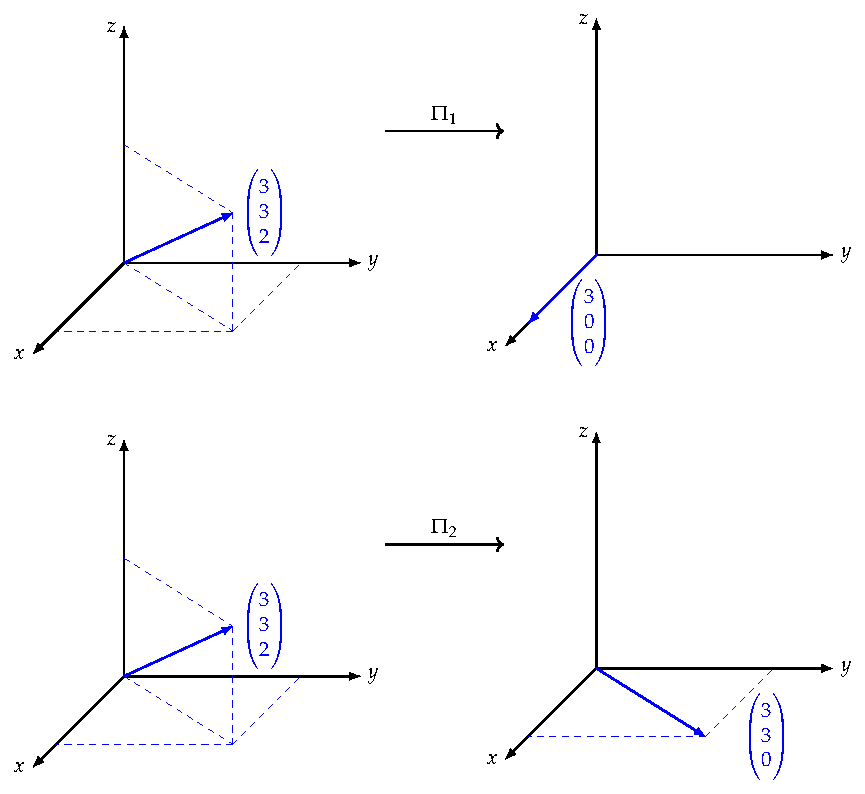
\includegraphics[]{Images/fig-projectorvisualization.pdf}
    \caption{Visualization of the action of projectors $\Pi_1, \Pi_2$ (as defined in Eq. \eqref{eq-projectorexamples}) on a vector in $\RR^3$. $\Pi_1$ can be visualized as projecting the given vector onto the one-dimensional subspace that is the $x$-axis subspace; preserving the $x$-component of the vector, and nullifying the $y$ and $z$-components. $\Pi_2$ can be visualized as projecting the given vector onto the two-dimensional subspace that is the $xy$-plane; preserving the $x$ and $y$ components of the vector and nullifying the $z$-component.}
    \label{fig-projectorvisualization}
\end{figure}

Now let's return to the bra-ket formalism and what projectors look like in this abstract setting. First, recall that we can write an observable $A$ in the form:
\begin{equation}
    A = \sum_i a_i \dyad{a_i}{a_i}
\end{equation}
where $\ket{a_i}$ is the eigenstate of $A$ corresponding to the eigenvalue $a_i$, and $\set{\ket{a_i}}_i$ is an ONB. In the non-degenerate case, each of the $a_i$s are distinct. However, in general degenerate eigenvalues (where $a_i = a_j$ for some $i, j$) are possible, and the current form of the expression does not make this particularly clear. With our knowledge of projectors, let us now rewrite the above as:
\begin{equation}
    A = \sum_a a \Pi_a
\end{equation}
where each of the $a$s are \emph{distinct} eigenvalues of $A$, and
\begin{equation}
    \Pi_a = \sum_{a_i = a} \dyad{a_i}{a_i}
\end{equation}
is the \emph{projector onto the eigenvalue-$a$ subspace}. Let us verify that these are indeed projectors. First, we verify that they are Hermitian:
\begin{equation}
    \Pi_a^\dagger = \left(\sum_{a_i = a} \dyad{a_i}{a_i}\right)^\dagger = \sum_{a_i = a} (\dyad{a_i}{a_i})^\dagger = \sum_{a_i = a} \dyad{a_i}{a_i} = \Pi_a.
\end{equation}
where in the second-to-last equality we use that $(\dyad{a}{b})^\dagger = \dyad{b}{a}$ (which follows immediately from the definition of the Hermitian adjoint; the proof is left to the reader!). Next, we show that they are idempotent (that is, they square to themselves):
\begin{equation}\label{eq-projectoridempotency}
    \Pi_a^2 = \left(\sum_{a_i = a} \dyad{a_i}{a_i}\right)^2 = \sum_{a_i = a} \sum_{a_j = a} \ket{a_i}\braket{a_i}{a_j}\bra{a_j} = \sum_{a_i = a}\sum_{a_j = a}\dyad{a_i}{a_j}\delta_{ij} = \sum_{a_i = a} \dyad{a_i}{a_i} = \Pi_a.
\end{equation}
So they are indeed projectors! In this form, we have decomposed the observable $A$ into the parts associated with each eigenvalue in a clear way. These projectors have some properties of note, described in the theorem below.

\begin{thmbox}{}
    Let $\set{\Pi_a}_a$ be the set of projectors associated to an observable $A$ (with $\Pi_a = \sum_{a_i = a}\dyad{a_i}{a_i}$ being the projector onto the eigenvalue-$a$ subspace). These projectors are mutually orthogonal:
    \begin{equation}\label{eq-projectororthogonality}
        \Pi_i\Pi_j = \delta_{ij}\Pi_i
    \end{equation}
    and are complete:
    \begin{equation}
        \sum_a \Pi_a = \II.
    \end{equation}
\end{thmbox}
\begin{proof}
    The idempotency of projectors covers the $i = j$ case in Eq. \eqref{eq-projectororthogonality}, and if $i \neq j$, then the expression is zero as eigenvectors of an observable $A$ corresponding to distinct eigenvalues are orthogonal. The completeness relation is merely a restatement of the resolution of the identity in terms of projectors.
\end{proof}

We are now ready to do our final, complete statement of the axioms of quantum measurement.

\begin{axiombox}{: Quantum measurement (version 3/final)}
    Let $A =  \sum_a a\Pi_a$ be the observable (a Hermitian operator) being measured,  where the $a$s are the eigenvalues of $A$ and $\set{\Pi_a = \sum_{a_i = a}\dyad{a_i}{a_i}}_a$ are the associated projectors onto the eigenvalue-$a$ subspaces. Let $\ket{\psi}$ be the pre-measurement state.

    \textbf{Dirac Postulate:} If outcome $a$ is measured, then the post measurement state is given by:
    \begin{equation}\label{eq-diracpostulate}
        \ket{\psi} \mapsto \frac{1}{\sqrt{\bra{\psi}\Pi_a\ket{\psi}}}\Pi_a\ket{\psi}.
    \end{equation}

    \textbf{Born rule:} The probability of measuring outcome $a$ is given by:
    \begin{equation}\label{eq-bornrule}
        p(a) = \bra{\psi}\Pi_a\ket{\psi}.
    \end{equation}
\end{axiombox}
We have now reproduced the form of the Dirac postulate and Born rule shown in the initial table! The above formulation of the measurement axiom(s) is very general, encompassing possible degenerate eigenvalues in the measured observables. Of course, it should be consistent with our previous statement of the axioms in the case that the eigenvalues are non-degenerate. It is highly recommended that you try this as an exercise first, but we will also give the argument here.

If an eigenvalue $a$ is non degenerate, then $\Pi_a = \dyad{a}{a}$. Eq. \eqref{eq-diracpostulate} then reads:
\begin{equation}\label{eq-diracconsistency}
    \ket{\psi} \mapsto \frac{1}{\sqrt{\braket{\psi}{a}\braket{a}{\psi}}}\ket{a}\braket{a}{\psi} = \frac{\braket{a}{\psi}}{\sqrt{\abs{\braket{a}{\psi}}^2}}\ket{a} = \frac{\braket{a}{\psi}}{\abs{\braket{a}{\psi}}} \ket{a} = e^{i\varphi}\ket{a} \sim \ket{a}.
\end{equation}
Which is consistent with the previous statement of the Dirac postulate. For the Born rule, we see that Eq. \eqref{eq-bornrule} reads:
\begin{equation}
    p(a) = \braket{\psi}{a}\braket{a}{\psi} = \abs{\braket{a}{\psi}}^2
\end{equation}
which is again consistent with our previous formulation.

The astute reader may object that we have seemingly ignored the possible complex phase factor sitting out front in Eq. \eqref{eq-diracconsistency}. However, this is not being sloppy, but instead a fact about quantum states that \emph{global phases are irrelevant}.

\begin{thmbox}{: Irrelevance of global phase}
    $\ket{\psi}$ and $\ket{\phi} = e^{i\varphi}\ket{\psi}$ correspond to the same physical quantum state.    
\end{thmbox}
\begin{proof}
    The two states are only distinct if we are able to distinguish them in a measurement. However, when calculating the probability of measuring an arbitrary outcome $a$ for any observable $A$ with the Born rule, we find that the two have identical measurement statistics:
    \begin{equation}
        p_{\phi}(a) = \bra{\phi}\Pi_a\ket{\phi} = \bra{\psi}e^{-i\varphi}\Pi_a e^{i\varphi}\ket{\psi} = \bra{\psi}e^{-i\varphi}e^{i\varphi}\Pi_a\ket{\psi} = \bra{\psi}\Pi_a\ket{\psi} = p_\psi(a).
    \end{equation}
    They therefore represent the same quantum state.
\end{proof}

We however note that \emph{relative} phases \emph{are} significant/relevant. For example, the $S_x$ eigenstates $\ket{+} = \frac{\ket{\uparrow} + \ket{\downarrow}}{\sqrt{2}}$ and $\ket{-} = \frac{\ket{\uparrow} - \ket{\downarrow}}{\sqrt{2}}$ differ by a relative phase, and are hence different quantum states.

Let us return to our motivating example with the spin-1 particle. We established that:
\begin{equation}
    S_z^2 = \hbar^2\left(\dyad{+}{+} + \dyad{-}{-}\right)
\end{equation}
has a degenerate eigenvalue, with both $\ket{+}$ and $\ket{-}$ being eigenstates with eigenvalue $+\hbar^2$. To deal with this degeneracy, we can use our new projector formalism of measurement. The projector corresponding to the $\hbar^2$ subspace is given by:
\begin{equation}
    \Pi_{\hbar^2} = \dyad{+}{+} + \dyad{-}{-}
\end{equation}
while the projector corresponding to the eigenvalue $0$ subspace is given by:
\begin{equation}
    \Pi_0 = \dyad{0}{0}.
\end{equation}
So, if we wanted to find the probability of measuring $S_z^2 = \hbar^2$ given a pre-measurement state $\ket{\psi}$, the probability would be given by:
\begin{equation}
    p(\hbar^2) = \bra{\psi}\Pi_1\ket{\psi} = \abs{\braket{+}{\psi}}^2 + \abs{\braket{-}{\psi}}^2
\end{equation}
and the post measurement state would be given by:
\begin{equation}
    \ket{\psi} \mapsto \frac{1}{\sqrt{\bra{\psi}\Pi_{\hbar^2}\ket{\psi}}}\Pi_{\hbar^2}\ket{\psi} = \frac{1}{\sqrt{\abs{\braket{+}{\psi}}^2 + \abs{\braket{-}{\psi}}^2}}\left(\braket{+}{\psi}\ket{+} + \braket{-}{\psi}\ket{-}\right).
\end{equation}

To conclude this section, we revisit the idea of individual vs. averaged measurement outcomes. We again consider the measurement of an observable $\sum_a a \Pi_a$. As before, the measurement outcomes of individual measurements are given by the eigenvalues $a$ of $A$. We can again calculate the average outcome/expectation value to be:
\begin{equation}
    \avg{A}_\psi \coloneqq \sum_a a p(a) = \sum_a a \bra{\psi}\Pi_a \ket{\psi} = \bra{\psi} \left(\sum_a a \Pi_a \right) \ket{\psi} = \bra{\psi} A\ket{\psi}
\end{equation}
so we see that Eq. \eqref{eq-expection2} holds as in the non-degenerate case.

\subsection{Compatible and Incompatible Observables}

\subsection{Position and Momentum}